Studies started at the Second World War because of the perfomance shortfalls and failures noted in manned equipment. These studies showed that these problems could diminish when Engineering, Psychology and Physiology were gathered when designing a system that was to be handled by a human being \cite{sandom2004human}.

This area of study was named "Human Factors" in United States an "Ergonomics" in Europe. Despite this difference in the names, today they are considered the same field of study. The International Ergonomics Association (IEA) defines Human Factors, and Ergonomics, as the following:

\begin{quote}
    Ergonomics (or human factors) is the scientific discipline concerned with the understanding of interactions among humans and other elements of a system, and the profession that applies theory, principles, data and methods to design in order to optimize human well-being and overall system performance. Human Factors professionals contribute to the design and evaluation of tasks, jobs, products, environments and systems in order to make them compatible with the needs, abilities and limitations of people \cite{karwowski2012discipline}.
\end{quote}

Besides being synonyms, this definition shows that humans is a variable inside a system and their interactions should be studied and that is the focus of Human Factors \cite{sandom2004human, sanders1998human, dul2003ergonomics}. 

Humans handle with devices, machines and equipment during their daily activities and all of these manipulations are susceptible to accidents or failures that can happen because of the interaction between operator, equipment and environment. Each interface with the operator can be a factor, for example:

\begin{itemize}
    \item The operator's body position during an activity;
    
    The position can impact on the comfort felled by the operator and this impacts on its concentration throughout the activity therefore impact on the success rate or in the chance of some accident happen \cite{sanders1998human}.
    
    \item The environment's lighting;
    
    The illumination can make details easier to be noted without provoking discomfort or distraction to the user and even increase productivity \cite{sanders1998human}.
    
    \item The information displayed and manipulation of the device.
    
    The way an information is displayed on a screen, figure or text impact on how efficient it will be understand by the operator. If this take too long it can draw the operator attention for too long and compromise his/her reaction time.
    
\end{itemize}

To take human into account when designing a product or a system is one of the principles for human factors \cite{sandom2004human} and the results of this human-centred-design is already a ISO Standard (BS EN ISO 13407 ‘Human-centred design processes for interactive systems’). This standard was originally written for computer-based-system, but easy applicable in other scenarios and areas \cite{sandom2004human}.

It is important to say that when it is said "User", it doesn't mean that one need to design a product specifically for an individual. The design has to be suited to everyone \cite{dul2003ergonomics}.

"Human-Machine systems" (on this thesis, for now on, called simply "Systems"), are interactions between humans and machines. These systems are designed to have an input, or demand, and an output, or product. Here, "machine" can be any manipulated object, from a simple screwdriver until a car, or some machine operated by more than one human, like a cargo ship for example. The Figure \ref{fig:human_machine_representaion} represent a general human-system machine interaction.

\begin{figure}[!htb]
    \centering

    \tikzstyle{arrow} = [rounded corners, line width = 1mm, bend left = 15, ->]
    
    \resizebox{0.85\width}{!}{
    \begin{tikzpicture}[node distance=1cm]
        
        \node (information) {
\includegraphics[width=.15\textwidth]{Fundamentação/Fatores Humanos/thinking.png}} 
        node(t_information)[below of = information,yshift=-0.75cm] {Information}
        node(t_information2)[below of = t_information,yshift=0.25cm] {processing};
        
        \node (controlling) [right of=information, xshift=5cm, yshift=-3cm] {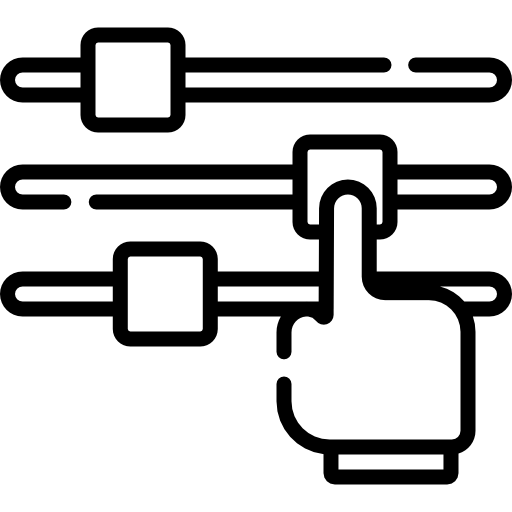
\includegraphics[width=.15\textwidth]{Fundamentação/Fatores Humanos/slider.png}}
        node(t_controlling)[below of = controlling,yshift = -0.75cm] {Controlling};
        
        \node (controls) [below of=controlling, yshift=-5cm,] {
\includegraphics[width=.15\textwidth,angle=90,origin=c]{Fundamentação/Fatores Humanos/control.png}} 
        node(t_controls) [below of = controls, yshift = -0.75cm]{Controls};
        
        \node (machine) [left of=controls, xshift=-5cm, yshift=-2cm] {
\includegraphics[width=.15\textwidth]{Fundamentação/Fatores Humanos/machine.png}} 
        node(t_machine) [below of = machine, yshift = -0.75cm]{Operation};
        
        \node (display) [left of=machine, xshift=-5cm, yshift=2cm] {
\includegraphics[width=.15\textwidth]{Fundamentação/Fatores Humanos/monitor.png}} 
        node(t_display) [below of = display, yshift = -0.75cm]{Display};
        
        \node (senses) [left of=information, xshift=-5cm, yshift=-2cm,] {\begin{tikzpicture}[node distance=1cm]
    \centering
    
    \node (eye) {
\includegraphics[width=.075\textwidth]{Fundamentação/Fatores Humanos/eye.png}};
    
    \node (ear) [right of=eye, yshift=-0.65cm] {
\includegraphics[width=.075\textwidth]{Fundamentação/Fatores Humanos/ear.png}};
    
    \node (nose) [left of=ear, yshift=-0.65cm] {
\includegraphics[width=.075\textwidth]{Fundamentação/Fatores Humanos/nose.png}};
    
    \node (hand) [right of=nose, yshift=-0.85cm] {
\includegraphics[width=.075\textwidth]{Fundamentação/Fatores Humanos/hand.png}};

\end{tikzpicture}} 
        node(t_senses) [below of = senses, yshift = -1.25cm]{Senses};
        
        \node (human) [below of=information, yshift=-4.75cm] {\Large{Human}};
        \node (human) [above of=machine, yshift=3.25cm] {\Large{Machine}};
        \node (human) [above of=information, yshift=1cm] {\Large{Work Environment}};
        
        \node (left_point) [left of=display, xshift=-2, yshift=2.75cm] {};
        \node (right_point) [right of=left_point, xshift=14cm] {};
        
        \node (input) [left of=machine, xshift=-5cm, yshift=-2cm] {\Large{Input}};
        \node (output) [right of=machine, xshift=5cm, yshift=-2cm] {\Large{Output}};
        
    
        \draw [arrow] (information.east) to (controlling.north west);
        \draw [arrow] (t_controlling.south) to (controls.north);
        \draw [arrow] (controls.west) to (machine.east);
        \draw [arrow] (machine.west) to (display.east);
        \draw [arrow] (display.north) to (t_senses.south);
        \draw [arrow] (senses.east) to (information.west);
        \draw [arrow] (input.east) -- (machine);
        \draw [arrow] (machine) -- (output.west);
        \draw [dashed,gray] (left_point) to (right_point);
        
        \draw (-8,-14) rectangle(8cm,1.5cm);
        
    \end{tikzpicture}
    }
    \caption{Human-Machine system representation \cite{sanders1998human}.}
    \label{fig:human_machine_representaion}
\end{figure}